To test whether word orders as found in natural language reflect optimization for the memory--surprisal tradeoff more generally, we compare the memory--surprisal tradeoffs of 54 actual languages to those of counterfactual baseline languages. These baseline languages differ from the actual languages only in their word order rules. This method of comparison against counterfactual baseline languages was introduced by \citet{gildea-optimizing-2007,gildea-grammars-2010} and has since been fruitfully applied to study optimization-based models of word order universals  \citep{futrell-large-scale-2015,gildea-human-2015,hahn2020universals}.

Here, we describe how we measure the memory--surprisal tradeoff in corpora, and how we generate counterfactual baseline languages. We then compare the tradeoff in real corpora against the tradeoff in the counterfactual baselines. For the majority of languages, we find that the real languages have more favorable memory--surprisal tradeoffs than the baselines, in line with the Efficient Tradeoff Hypothesis.

\subsection{Measuring the memory--surprisal tradeoff in corpora}

The key to evaluating the memory--surprisal tradeoff from corpus data is the set of quantities $I_t$, the  mutual information between words at distance $t$ conditional on the intervening words. % (defined in Section~\ref{sec:ms-tradeoff}). 
These quantities can be plugged in to Theorem~\ref{prop:suboptimal} to give a lower bound on the memory--surprisal tradeoff.

The quantities $I_t$ can be estimated as the difference between the average surprisal of Markov models that have access to the last $t-1$ or $t$ words.
That is, if we have a $t$th-order Markov model with average surprisal
\begin{equation*}
    S_t = H[w_t | w_0, \dots, w_{t-1}]
\end{equation*}
and a $(t-1)$th-order Markov model with average surprisal
\begin{equation*}
    S_{t-1} = H[w_t | w_1, \dots, w_{t-1}],
\end{equation*}
then we can calculate $I_t$ straightforwardly in the following way:
\begin{align}
    \nonumber
    I_t &= I[w_t : w_0 | w_1, \dots, w_{t-1}] \\
    \nonumber
    &= S_{t-1} - S_t.
\end{align}
Therefore, to evaluate $I_t$, all we need is a way of fitting Markov models of order $t$ and $t-1$ and computing their average surprisals.

To fit Markov models to the data, we use neural language models. In particular, we use Recurrent Neural Networks with Long Short-Term Memory architectures \citep{hochreiter-long-1997}. 
Neural network models are the basis of the state-of-the art in statistical modeling of language. Surprisal estimates derived from such models have been shown to best predict reading times, compared to other models, e.g., n-gram models~\citep{frank-insensitivity-2011,goodkind-predictive-2018}.
See SI Section 3.2 for details on how these models were fit to data, and see SI Sections 3.4 and 3.5 for control studies using other methods of estimating $I_t$ (based on $n$-gram models and PCFG chart parsers). These control studies yield the same qualitative results as the neural network-based studies presented here.

For each language, we run the neural network estimator multiple times with different random seeds, to control for variation in the random initialization of model parameters (see SI Section 3.2.3 for details).

In order to evaluate the average surprisal values $S_t$, we computed the empirical word-by-word surprisal values under the $t$th-order Markov model for held-out data, different from the data that was used to train the model. By evaluating on held-out data, we avoid underestimating the value of $S_t$ due to overfitting.
We chose held-out data based on existing splits of corpora, see section `Data' below.




\subsection{Data}\label{sec:exp2-data}
We draw on syntactically annotated corpora, compiled by the Universal Dependencies project for several dozen languages~\citep{nivre-universal-2017}.
These are annotated in the format of Dependency Grammar~\citep{hays1964dependency,hudson1984word,melcuk1988dependency,corbett1993heads,tesniere2015elements}.
In such dependency corpora, sentences are annotated with \emph{dependency trees} (Figure~\ref{fig:dependency}).
These are directed trees describing the grammatical relations among words. For example, the arcs labeled ``obj'' represent that the noun in question is the \emph{direct object} of the verb, rather than e.g. the subject or an indirect object.
A dependency arc is drawn from a \emph{head} (e.g. the verb `has') to a \emph{dependent} (e.g. its object `book').
Dependency trees can be defined in terms of many different syntactic theories \citep{corbett1993heads}.
Although there are some differences in how different formalisms would draw trees for certain sentences, there is broad enough agreement about dependency trees that it has been possible to develop large-scale dependency-annotated corpora of text from dozens of languages \citep{nivre2017universal}.

\begin{figure}
\centering
\begin{dependency}[theme = simple]
   \begin{deptext}[column sep=1em]
Mary \&	 has \& two \& green \& books  \\
   \end{deptext}
	%   \depedge[edge start x offset=-6pt]{2}{5}{ATT}
	%   \deproot{3}{ROOT}
   \depedge{2}{1}{nsubj}
   \depedge{2}{5}{obj}
   \depedge{5}{3}{nummod}
   \depedge{5}{4}{amod}
   %\depedge[arc angle=50]{7}{6}{ATT}
\end{dependency}
	\caption{An English sentence with dependency annotations, according to the Universal Dependencies 2.4 standard \citep{nivre-universal-2017}.
	We visualize grammatical relations as arcs drawn from heads (e.g., the verb `has') to dependents (e.g., its object `book').
	}\label{fig:dependency}
\end{figure}

%\paragraph{Selection of Languages}
We computed memory--surprisal tradeoffs for all languages for which there are Universal Dependencies 2.4 treebanks with a total of at least 500 sentences of training data.
We excluded data from historical languages, as these corpora often include poetry, translated text, or texts spanning several centuries.\footnote{Historical languages excluded: Ancient Greek, Classical Chinese, Coptic, Gothic, Latin, Old Church Slavonic, Old French.}
This resulted in 54 languages.

%\paragraph{Processing of Corpora}
For each of these languages, we pooled all available corpora into one dataset.
We excluded corpora that primarily contain code-switched text\footnote{Hindi English corpus} or text created by non-native speakers.\footnote{ESL for English, CFL for Chinese.}
Most Universal Dependencies corpora have a predefined split into \emph{training}, \emph{held-out} (also known as \emph{development}), and \emph{test} partitions.
%While larger corpora have all three partitions, smaller corpora often have only some of these partitions.
In most cases, we used the predefined data split, separately pooling data from the different partitions. 
For some languages with little data, there is no predefined training partition, or the training partition is smaller than the other partitions.
In these cases, we redefined the split to obtain more training data.
For these languages, we pooled all the available partitions, used 100 randomly selected sentences as held-out data, and used the remainder as training data.\footnote{This affects Amharic, Armenian, Breton, Buryat, Cantonese, Faroese, Kazakh, Kurmanji, Naija, Thai, and Uyghur.}
We did not make use of the \textit{test} partitions here.
We provide the sizes of the resulting datasets in SI Section 3.1.
The datasets ranged in size from 564 sentences (Armenian) to 114,304 sentences (Czech), with a median of 5,255 sentences per language.
For each language, we obtain a stationary process by concatenating the sentences from the corpus in random order, separated with an end-of-sentence symbol.


\subsection{Defining baselines}\label{sec:baselines}

Testing the Efficient Tradeoff Hypothesis requires comparing the memory--surprisal tradeoffs of real grammars to those of baseline grammars. The baseline grammars we construct are counterfactual ordering grammars that define consistent ordering rules similar to those found in actual languages (Figure~\ref{fig:grammars}).
For instance, these grammars specify which dependents precede or follow their heads (e.g., whether objects follow or precede verbs, whether adjectives follow or precede nouns), and the relative order of different dependents on the same side of the head (e.g., whether noun phrases have order adjective-numeral-noun or numeral-adjective-noun). Our formalism of ordering grammars was introduced in \citet{hahn2020universals}, adapting the method of \citet{gildea-optimizing-2007,gildea-grammars-2010,gildea-human-2015} to the setting of dependency corpora.


\begin{figure}
\centering
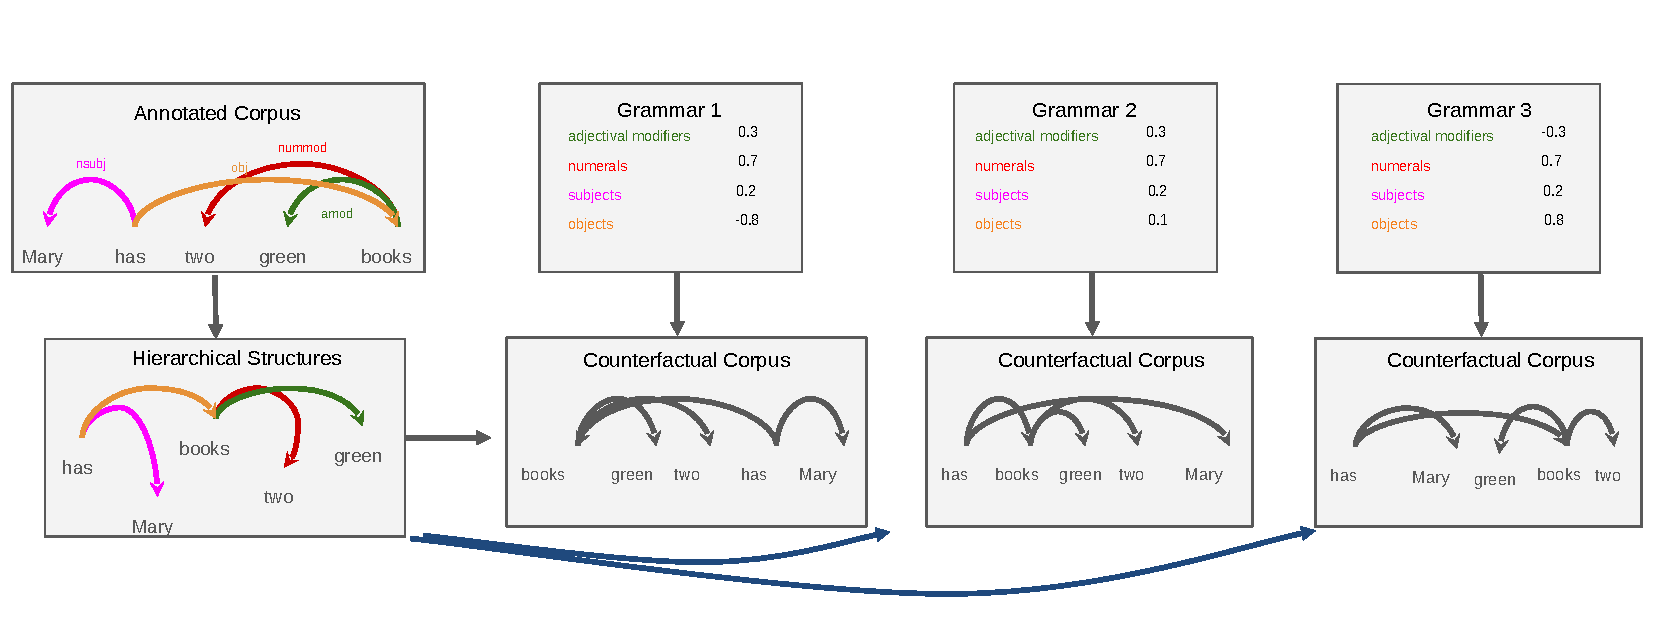
\includegraphics[width=\textwidth]{figures-gdrive/counterfactual-languages.pdf}
\caption{Estimating chance by constructing counterfactual grammars and languages: We start from an annotated dependency corpus of sentences annotated with syntactic dependencies (top left). We then extract the raw dependency structures, stripping away word order information (bottom left).
We construct baseline ordering grammars that provide rules for ordering the words in such dependency structures (Grammars 1--3).
Applying any such grammar to the dependency structures yields a counterfactual corpus of a hypothetical language that has the same dependency structures as the actual language, but different word order rules.}\label{fig:grammars}
\end{figure}


Universal Dependencies 2.4 defines 37 universal syntactic relations that are used to label dependency arcs across all corpora.
These relations encode cross-linguistically meaningful relations such as subjects (\textit{nsubj}, see Figure~\ref{fig:dependency}) , objects (\textit{obj}), and adjectival modifiers (\textit{amod}).
We define ordering grammars by assigning a parameter $a_\tau \in [-1,1]$ to every one of these 37 universal syntactic relations.
Relations sometimes have language-specific subtypes; we do not distinguish these subtypes.
Following Gildea and colleagues, this parameter defines how dependents are ordered relative to their head:
Given a head and a set of dependents, we order each dependent by the parameter $a_\tau$ assigned to the syntactic relation linking it to the head.
Dependents with negative weights are placed to the left of the head; dependents with positive weights are placed to the right. Ordering grammars describe languages that have consistent word order.
For instance, the subject is consistently ordered before or after the verb, depending on whether the parameter $a_{nsubj}$ for the verb-subject dependency is positive or negative.

We constructed baseline grammars by randomly sampling the parameters $a_\tau$.
Such baseline grammars define languages that have consistent word order but, crucial for our purposes, do not exhibit systematic preferences for specific word order patterns such as short dependencies.

We first constructed at least 10 baseline grammars for each of the 54 real languages.
We then continued to construct baseline grammars until a precision-based stopping criterion was reached. This criterion was designed to ensure that enough grammars were sampled to reliably compare the tradeoff curves of real and baseline grammars, without biasing results towards or against our hypothesis (see SI Section 3.2.3).
The stopping criterion compared what fraction of baseline grammars had strictly more (or strictly less) efficient tradeoff curves than the real ordering, and required a bootstrapped 95\% confidence interval for that ratio to have width $\leq 0.15$.
The resulting number of baseline grammars ranged from 10 (Italian and Romanian) to 347 (Estonian).\footnote{Due to a scripting error, 846 grammars were generated for Erzya even though this was not required by the stopping criterion.}

Due to the way ordering grammars are specified, certain kinds of rules cannot be modeled by our word order grammars.
This includes rules sensitive to the category of the dependent, such as the difference between postverbal nominal objects and preverbal pronominal objects in Romance languages.
It also includes rules sensitive to larger context, e.g., the alternation between verb-final order in embedded clauses and verb-initial/verb-medial order in main clauses in German and Dutch.
Furthermore, the model does not allow rules specifying interactions between different constituents, for instance, verb-second order, where exactly one dependent precedes the verb, and all others follow it.
Finally, the model does not account for word order freedom, as all ordering choices are deterministic.
In this sense, ordering grammars only represent an approximation to the kinds of ordering rules found in natural language \citep{gildea-optimizing-2007, gildea-grammars-2010, gildea-human-2015}.
Other models described in the literature \citep{futrell2015experiments, wang2016galactic} mostly share these limitations.


To ensure that results are not due to the representational restrictions of the word order grammar formalism, we also compared the baselines to the result of ordering the corpora according to grammars that approximate the real orders to the extent possible in the grammar formalism.
These grammars have exactly the same representational constraints as the baseline grammars while approximating the real orderings.
We expect these grammars to have better memory--surprisal tradeoffs than comparable random baseline grammars across all languages.
We created these ordering grammars by fitting them to the actual orderings of each language using the method of \cite{hahn2020universals}.
They match the order of the actual language in those cases where order of a relation is fully consistent; for relations where order is variable, they approximate this by modeling the most frequent order.
In representing word order rules, they have the same limitations as baseline grammars have, for instance, they cannot specify rules sensitive to the category of the dependent or to larger context.


\subsection{Results}\label{sec:main-experiment-results}
To test the Efficient Tradeoff Hypothesis, we compare the tradeoff curves for the real orders with those for random baseline grammars.
In Figure~\ref{fig:it}, we show the estimated values of $I_t$ for real and fitted orders and the median of $I_t$ across different baseline grammars.
In most languages, $I_1$ is distinctly larger for the actual and fitted orderings compared to the baseline orderings. This means that real orderings tend to concentrate more predictive information at the immediately preceding word than baseline grammars.

In Figure~\ref{fig:median-table-expt2}, we show the resulting bounds on the memory--surprisal tradeoff curves, showing surprisals at given levels of memory, for real and baseline languages.
We compute surprisal at 40 evenly spaced points of memory (selected individually for each language, between 0 and the maximal memory capacity $H_M$ obtained using Theorem~\ref{prop:suboptimal}), over real orders and baseline grammars.
At each point, we then compute the median surprisal over all model runs for the real language, and over all baselines grammars.
For each point, we compute an non-asymptotic and non-parametric 95\% confidence interval for this median surprisal using the binomial test.

Numerically, the real language provides a better tradeoff than the median of the baselines across all languages, with four exceptions (Latvian, North Sami, Polish, Slovak). In order to quantify the degree of optimality of real orders, we further computed the area under the memory--surprisal tradeoff curve (AUC) for real and baseline orderings.
Area under the curve (AUC) is a general quantity evaluating the efficiency of a tradeoff curve \citep{bradley1997use}.
A \emph{smaller} area indicates a \emph{more efficient} memory--surprisal tradeoff.
In Figure~\ref{fig:auc}, we plot the AUC for the real orderings, together with the distribution of AUCs for baseline grammars.
We quantify the degree of optimality by the fraction of baseline grammars for which the AUC is higher than for the real orders:
The real ordering is highly efficient if it results in a lower AUC than almost all baseline grammars.
Numerically, the AUC is smaller in the real orderings than in at least 50\% of baseline grammars in all but three languages (Polish, Slovak, North Sami).
We evaluated significance using a two-sided binomial test.
In these three languages, the AUC is higher in the real orderings than in significantly less than 50\% ($p < 0.01$ in each language).
In all other languages except for Latvian, the fraction of more efficient baseline grammars was significantly less than 50\%, at $p=0.01$, where we applied Hochberg's step-up procedure \citep{hochberg1988sharper} to control for multiple comparisons.
In 42 of the 54 languages, the real language was more efficient than all of the sampled baseline grammars. % fraction of more efficient baseline grammars out of the samples taken was 0\%.



The AUC for the fitted grammars is lower than more than 50\% of random baseline grammars in all 54 languages ($p < 0.01$, using two-sided Binomial test and Hochberg's step-up procedure). Thus, we replicate the result that ordering regularities of real languages provide more efficient tradeoffs than most possible order grammars even when comparing within the same word order grammar formalism.



\definecolor{baseline}{HTML}{00BA38}
\definecolor{real}{HTML}{619CFF}
\definecolor{fitted}{HTML}{F8766D}

\begin{figure}
	\begin{center}
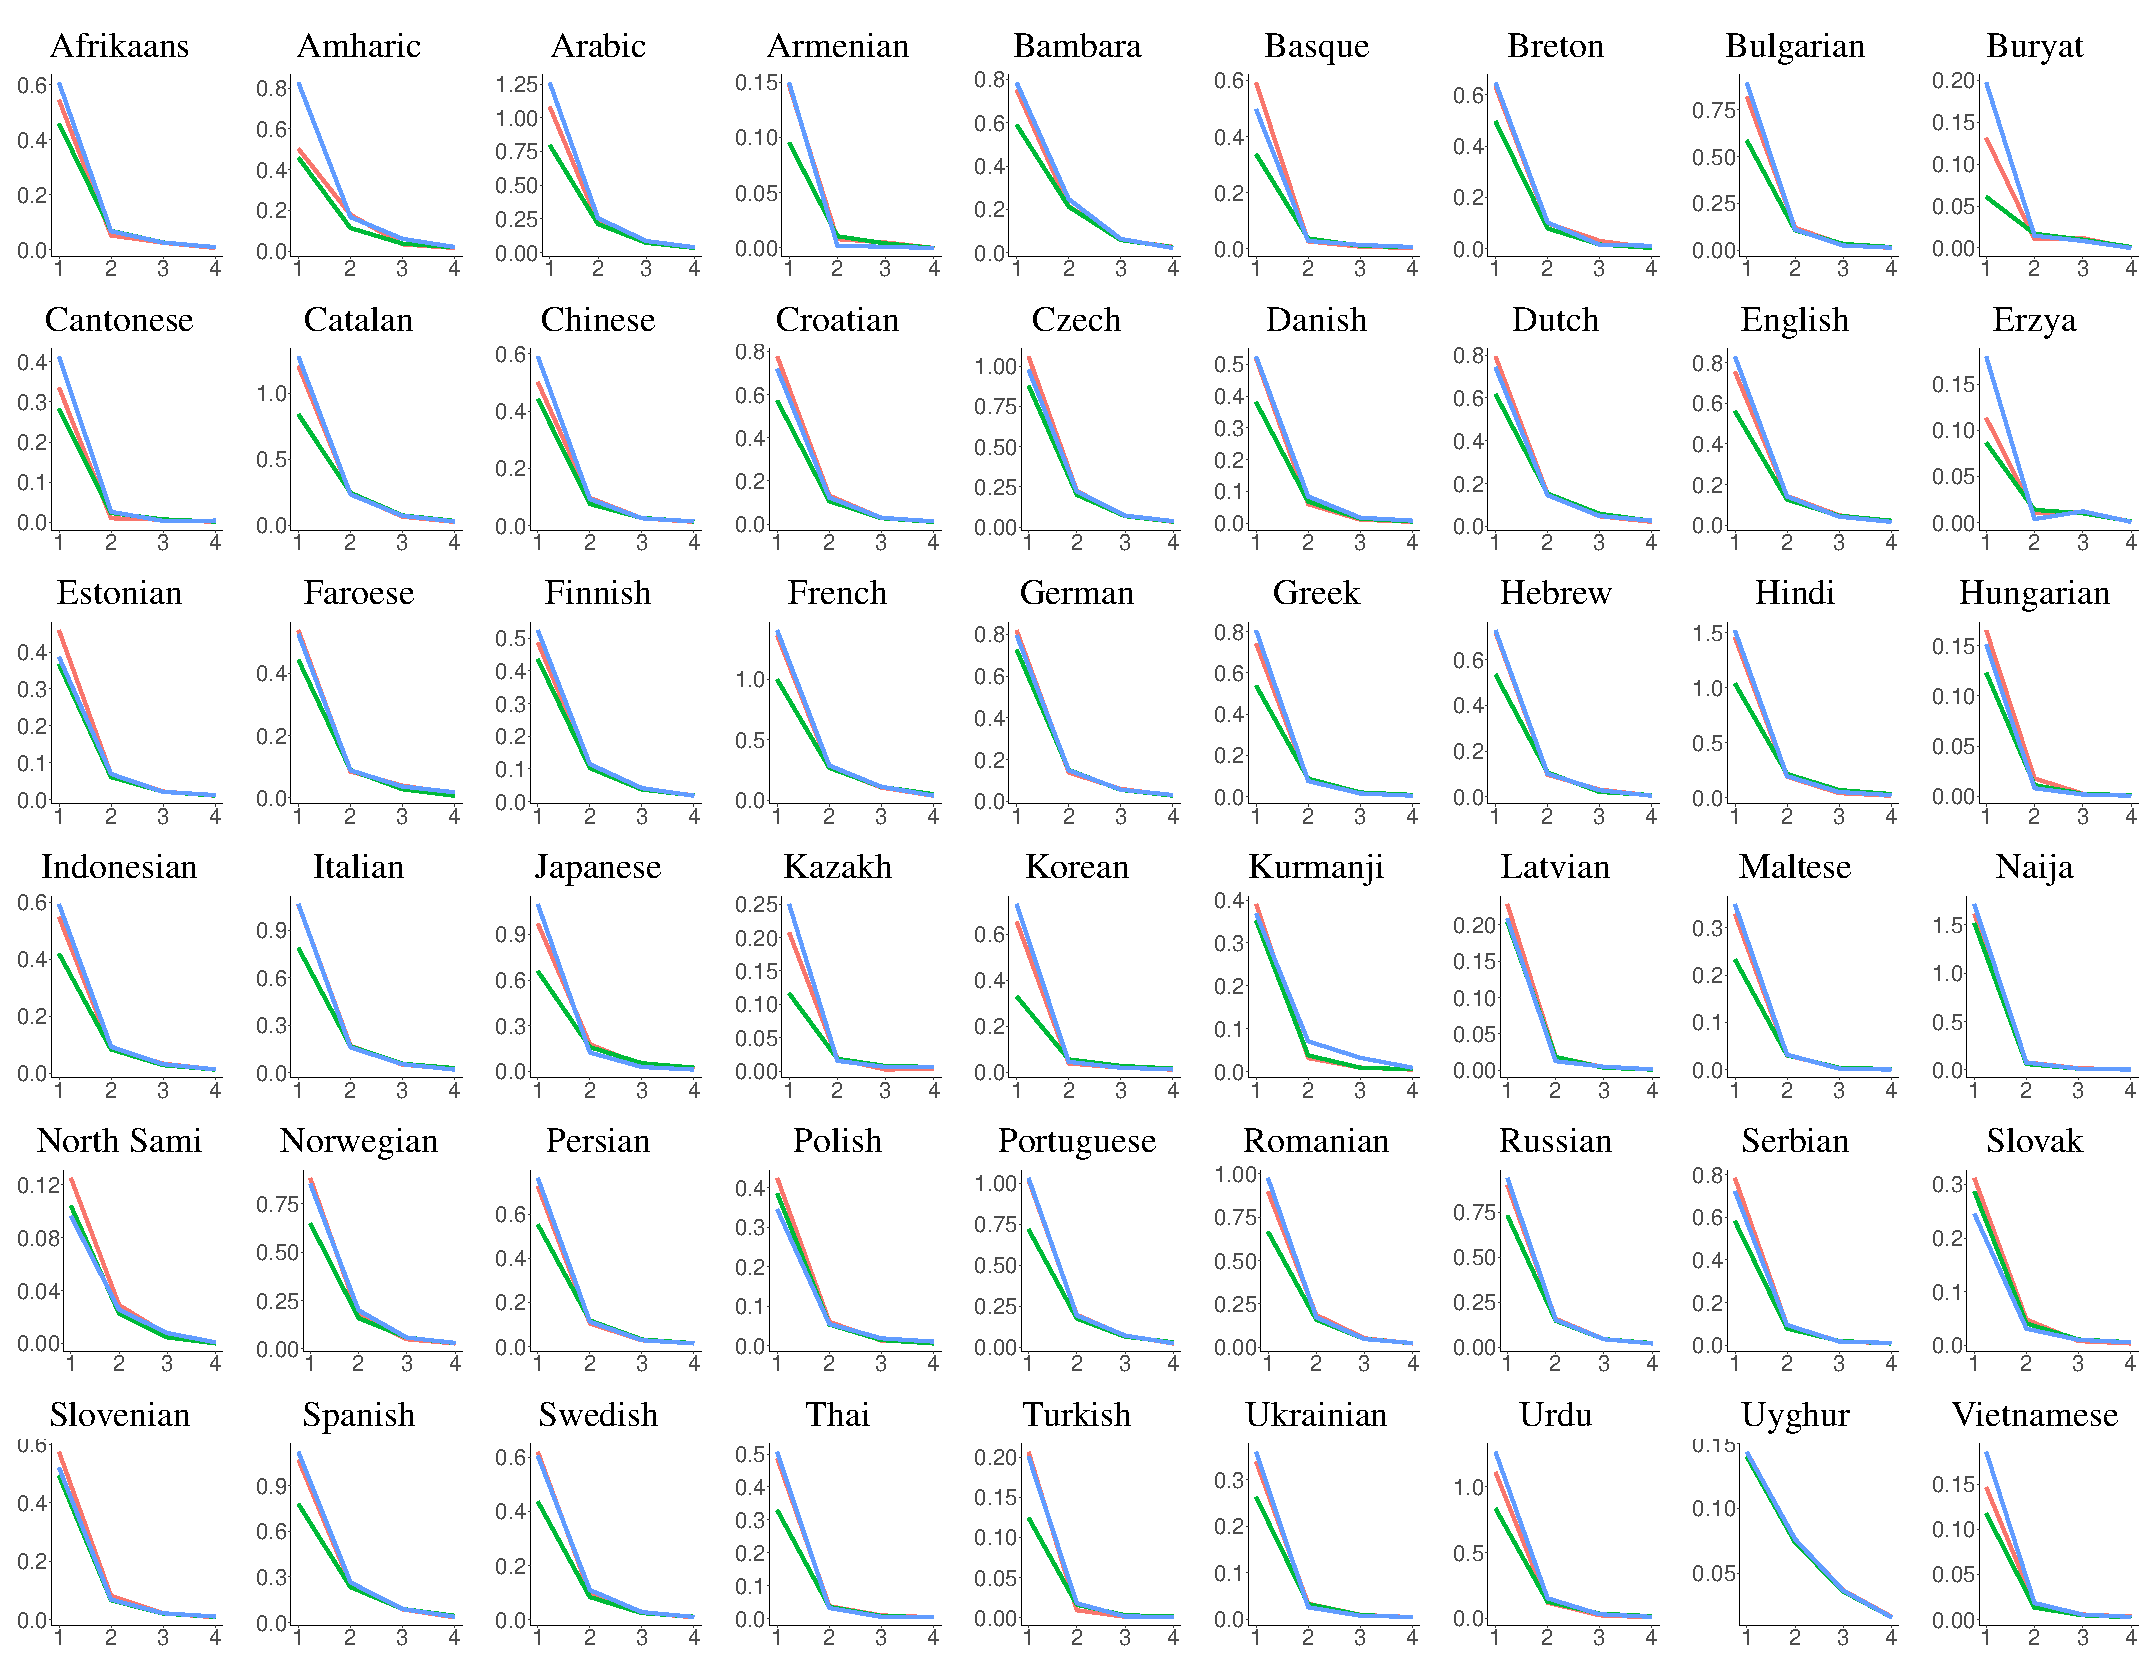
\includegraphics[width=\textwidth]{it-table-mle.pdf}
\end{center}

\begin{center}
\begin{tabular}{llll}
\textbf{\textcolor{fitted}{----}} Fitted&
\textbf{\textcolor{real}{----}} Real&
\textbf{\textcolor{baseline}{----}} Baselines&
\end{tabular}
\end{center}
\caption{Conditional mutual information $I_t$ (y-axis) as a function of $t$ (x-axis), for real (blue), fitted (red) and baseline (green) orders. We plot the median over all sampled baseline grammars.}\label{fig:it}
\end{figure}



\begin{figure}
	\begin{center}
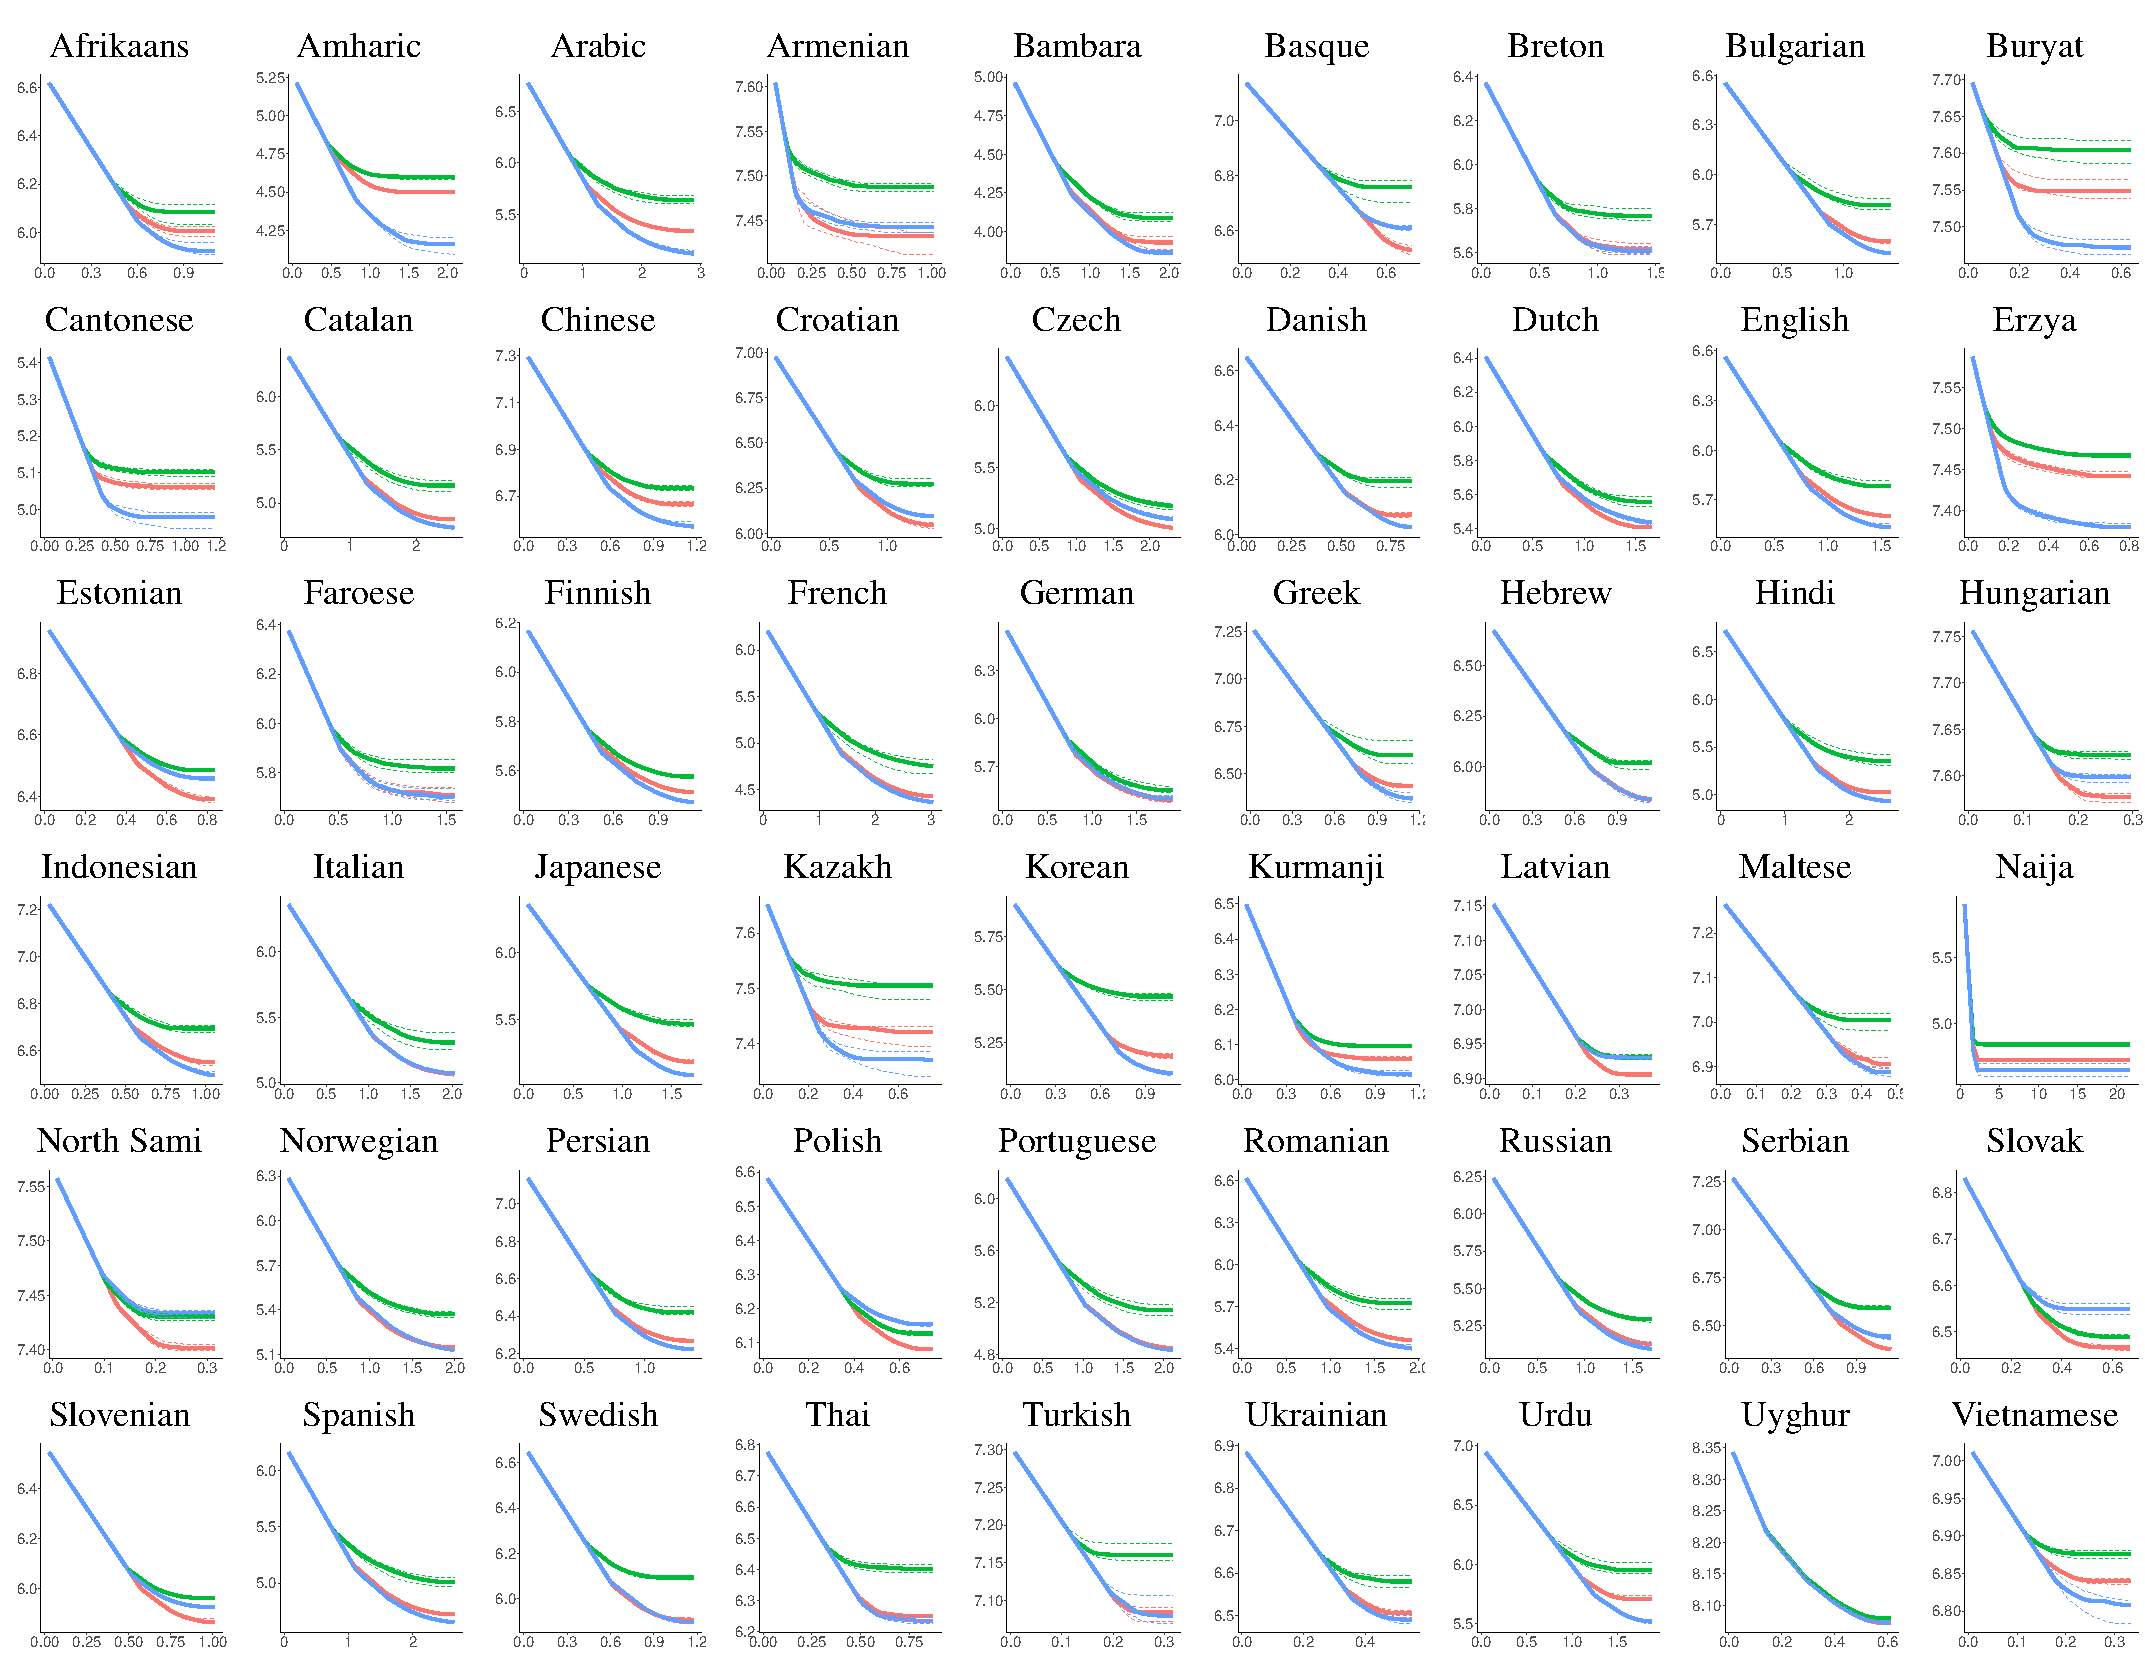
\includegraphics[width=\textwidth]{results-table-mle.pdf}
\end{center}

\begin{center}
\begin{tabular}{llll}
\textbf{\textcolor{fitted}{----}} Fitted&
\textbf{\textcolor{real}{----}} Real&
\textbf{\textcolor{baseline}{----}} Baselines&
\end{tabular}
\end{center}
	\caption{Surprisal (y-axis) at given memory level (x-axis), for real (blue), fitted (red), and baseline (green) orders.
	For the real (blue) and fitted (red) orders, we provide the median across multiple random seeds of the neural network estimator for $I_t$ (see SI Section 3.2.2), and 95\% confidence bands.
	For the baseline grammars (green), we provide the median across both the sampled baseline grammars and multiple random seeds of the estimator, and 95\% confidence bands for this median.
}\label{fig:median-table-expt2}
\end{figure}


\begin{figure}
	\begin{center}
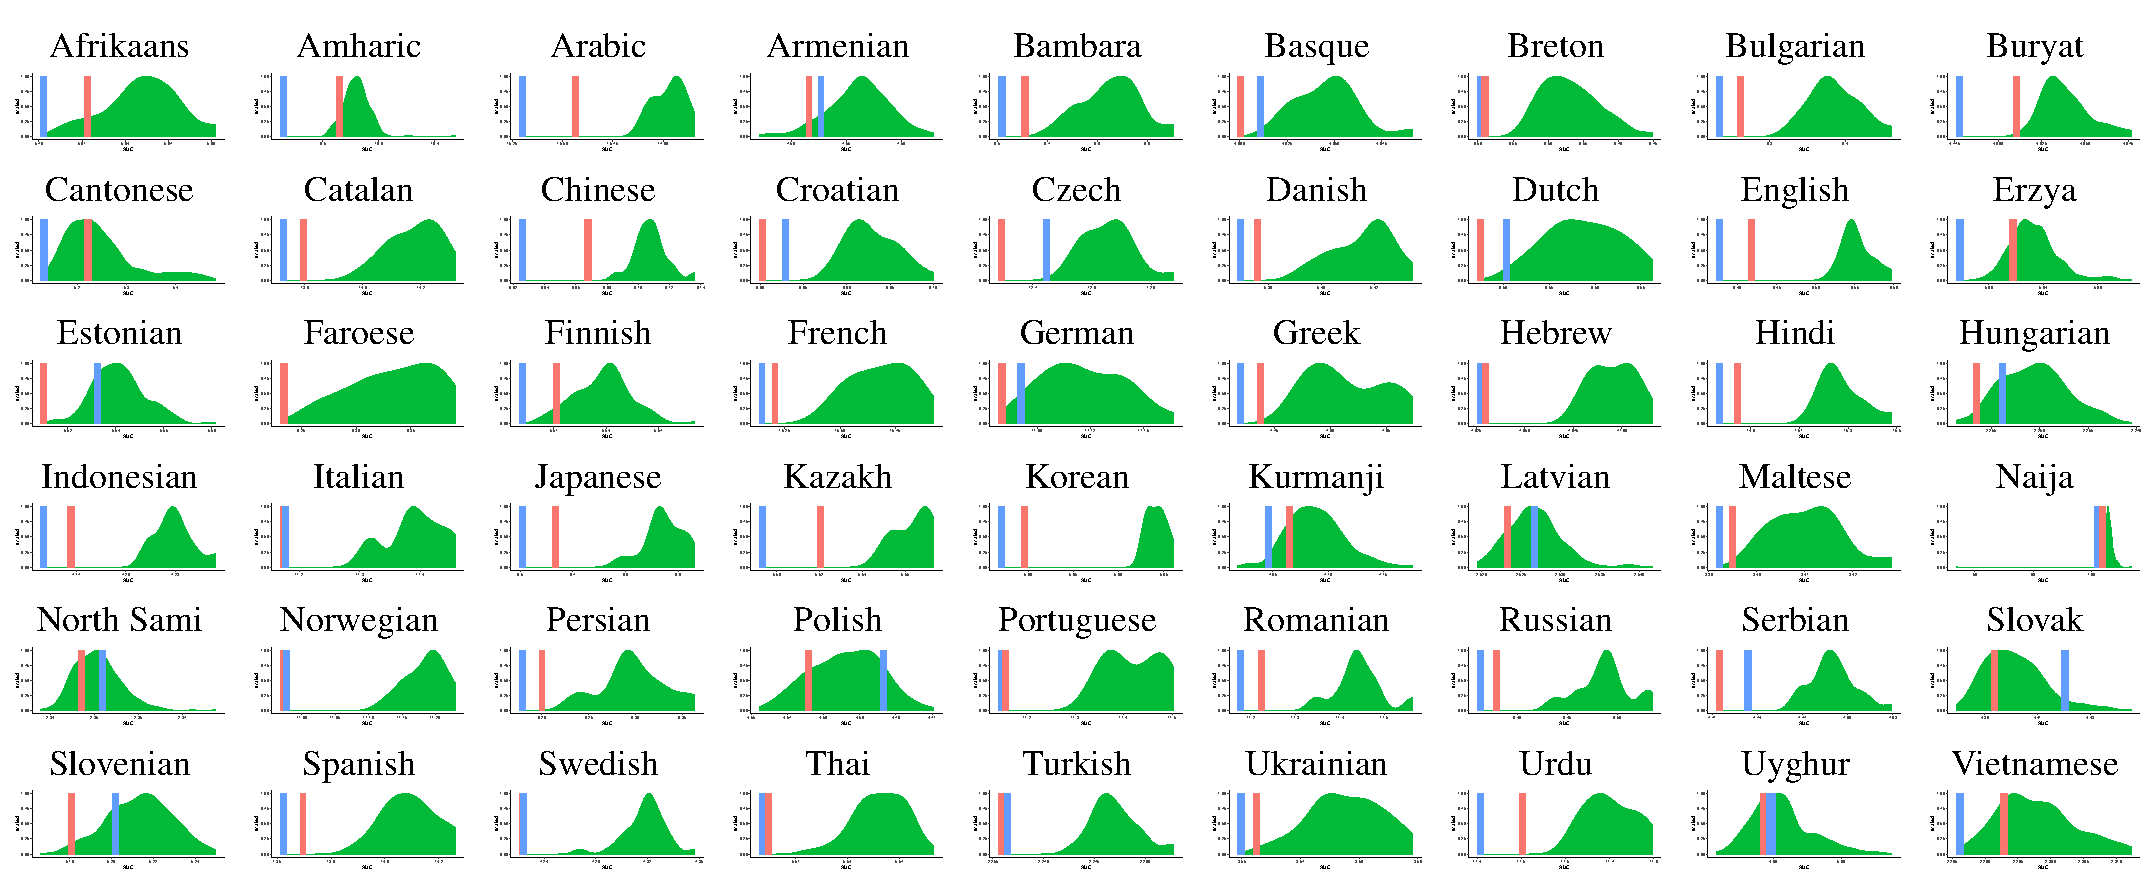
\includegraphics[width=\textwidth]{auc-table_MLE.pdf}
\end{center}

\begin{center}
\begin{tabular}{llll}
\textbf{\textcolor{fitted}{----}} Fitted&
\textbf{\textcolor{real}{----}} Real&
\textbf{\textcolor{baseline}{----}} Baselines&
\end{tabular}
\end{center}
\caption{Histograms for the Area under the Curve (AUC) for the memory--surprisal tradeoffs for real (blue), fitted (red), and random (green) orders.
We provide a kernel density smoothing estimate of the distribution of random baseline orders.
A smaller AUC value indicates a more efficient tradeoff.
In most cases, the real and fitted orders provide more efficient tradeoffs than most or all baseline grammars.
}\label{fig:auc}
\end{figure}




\subsection{Discussion}\label{subsec:expt2-discussion}

We have found that 50 out of 54 languages provide better memory--surprisal tradeoffs than random baselines with consistent but counterfactual word order rules.
Four languages provide exceptions; these are Latvian (Baltic), North Sami (Uralic), Polish and Slovak (both Slavic). These four languages did not have significantly lower AUC values than half of the random baselines.
One feature that unites these four languages is that they have strong word order freedom, as we will see below in Figure~\ref{fig:freedom-surp}. % \mhahn{(also CITE something)}.
Word order freedom plausibly makes sentences less predictable, as the same syntactic structure can receive different surface realizations.
We thus hypothesized that word order freedom  impacts the memory--surprisal tradeoff, and that languages with more strongly fixed word order should display more optimal memory--surprisal tradeoffs.


To test this hypothesis, we examined the correlation between word order freedom and the surprisal difference between real and baseline orderings.
To quantify word order freedom, we used a corpus-based estimate, the \key{branching direction entropy}~\citep{futrell-quantifying-2015}.
This is the entropy of the ordering (head-first or dependent-first) of dependencies conditioned on the dependency label and the part-of-speech label of head and dependent.
These two quantities are plotted in Figure~\ref{fig:freedom-surp}.
We found that branching direction entropy was strongly correlated with the surprisal difference between real and baseline orderings (Spearman correlation $-0.58$, $p < .0001$).

This result might mean that optimization of word orders for memory--surprisal tradeoffs is indeed stronger in languages with more fixed word order, and that word order freedom leads to less efficient memory--surprisal tradeoffs.
A second possibility is that languages with seemingly free word order encode other information in word order, in particular, information about information structure \citep[e.g.][]{givon1988pragmatics,firbas1966defining,firbas1974aspects,myhill1985pragmatic}.
Next, we test the latter hypothesis by examining whether the degree of optimization changes when taking into account information structure.




\begin{figure}
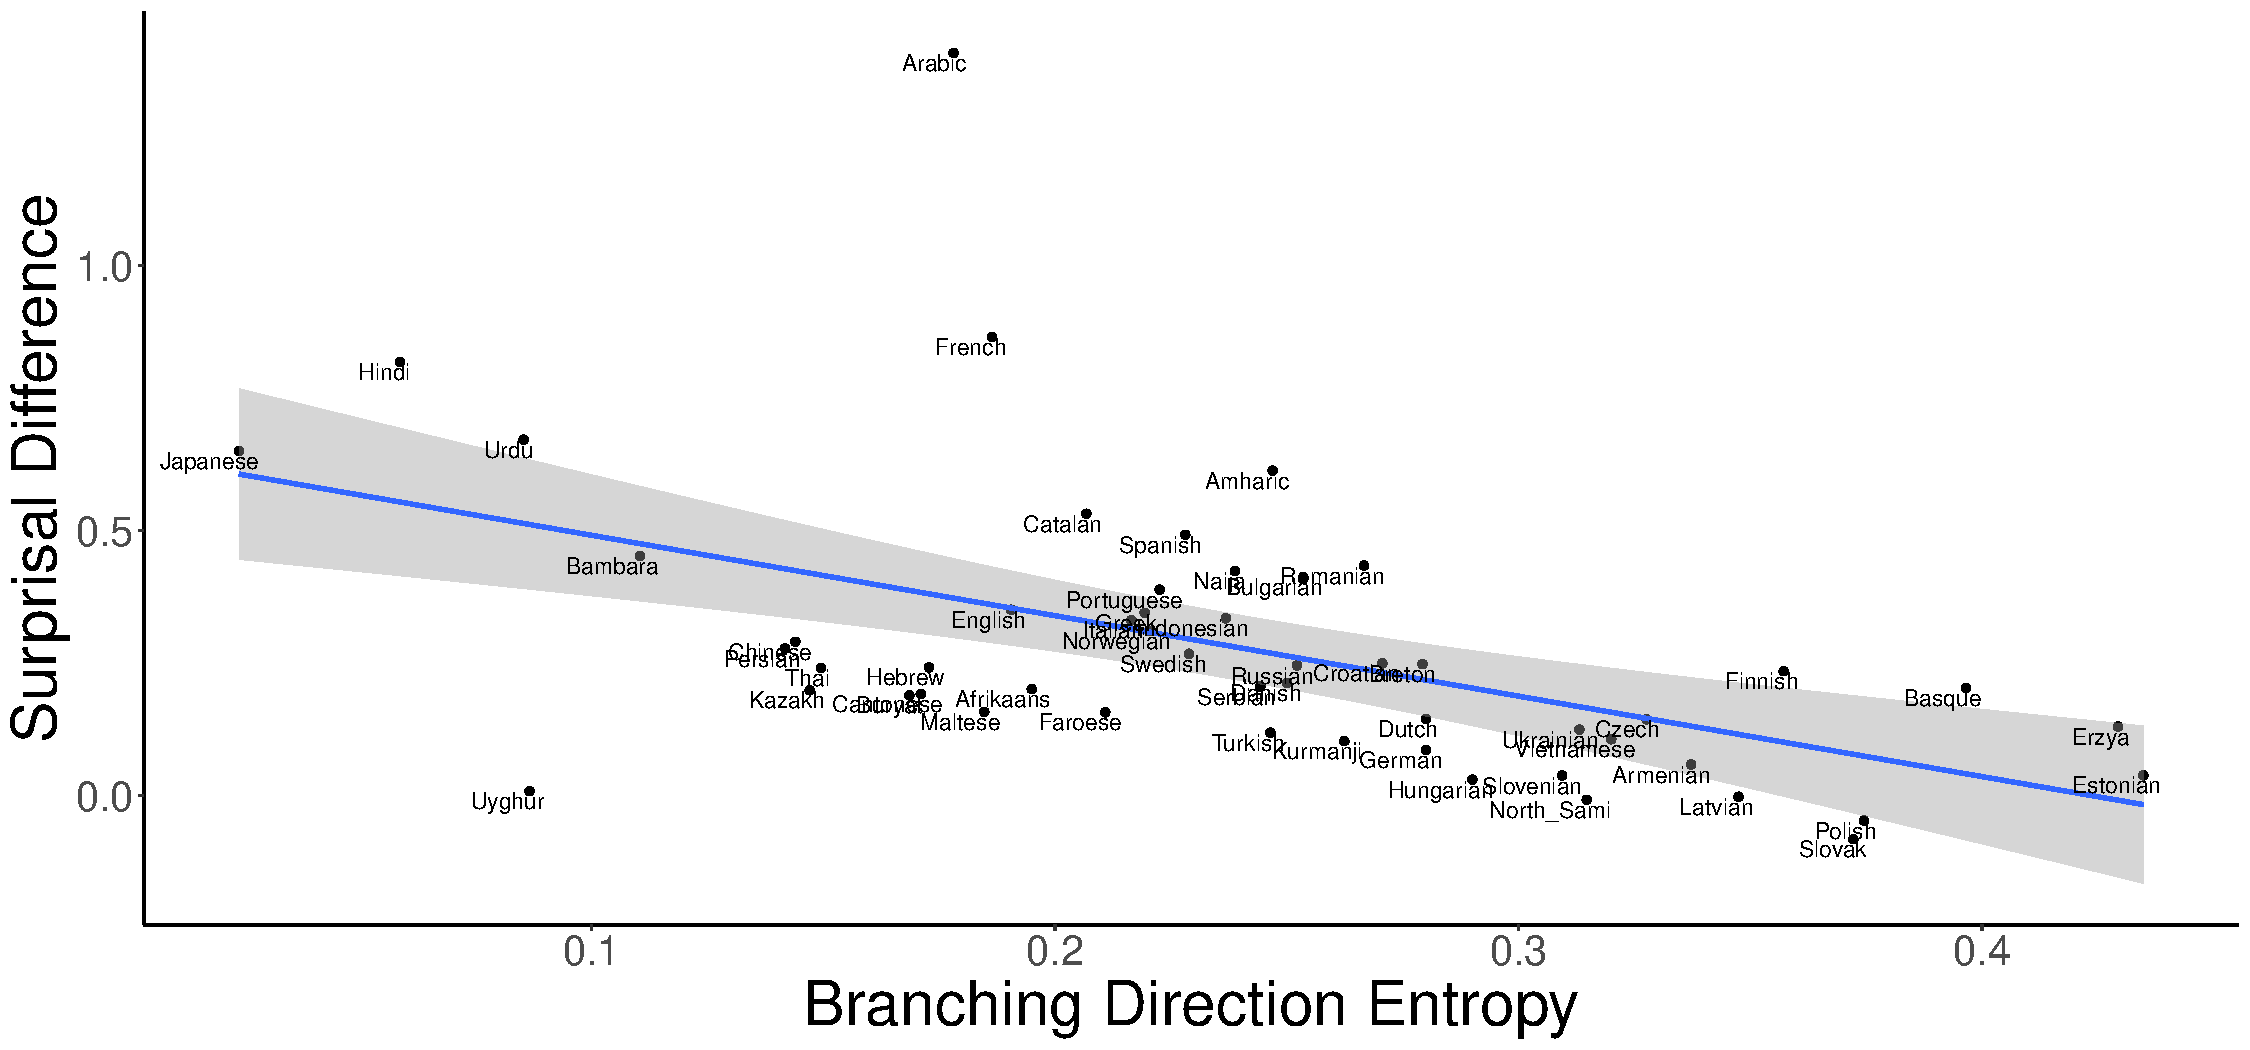
\includegraphics[width=0.95\textwidth]{figures/surprisal-branching-entropy-REAL-invert.pdf}
	\caption{Word order freedom and strength of optimization: For each of the 54 languages, we show word order freedom as measured by branching entropy, and the difference between the real order's surprisal and the median surprisal of the baseline grammars, at the maximum memory value (see Figure~\ref{fig:median-table-expt2}).
	Languages with higher branching direction entropy show a smaller reduction in surprisal compared to baseline orders.\jd{the languages are printed in very low resolution -- not sure if this is an issue with the plot or with my monitor. ideally the labels would generally be a little bigger. you can use the ggrepel package to make sure labels don't overlap}
	}\label{fig:freedom-surp}
\end{figure}



